\documentclass[9pt,aspectratio=169]{beamer}

\usetheme{Madrid}
\usecolortheme{default}
\usefonttheme{professionalfonts}

\setbeamertemplate{navigation symbols}{}
\setbeamertemplate{footline}[frame number]
\setbeamercolor{block title}{bg=blue!20,fg=black}
\setbeamercolor{block body}{bg=blue!5,fg=black}

\usepackage[utf8]{inputenc}
\usepackage{amsmath}
\usepackage{booktabs}
\usepackage{array}
\usepackage{graphicx}
\usepackage{adjustbox}
\usepackage{tikz}
\usetikzlibrary{arrows.meta,positioning,shapes.geometric}

\title[MyHealthReport -- Platform Plan]{MyHealthReport}
\subtitle{Platform Structure \& Execution Plan\\ \small Website, desktop and mobile architecture, technology stack,\\ feature scope, and the medical department's execution plan}
\author{}
\date{28 August 2026}

\begin{document}

\begin{frame}
\titlepage
\end{frame}

\begin{frame}{Agenda}
\tiny
\tableofcontents
\end{frame}

\section{One Core, Three Front Ends}

\begin{frame}[t]{One Core, Three Front Ends}
\textcolor{black!55}{\scriptsize A single source of truth behind every channel}\\[2pt]
\begin{itemize}
\scriptsize
\item Medical knowledge is never hard-coded into a client -- all three versions are front ends over the \emph{same} backend
\item Website, desktop, and mobile call the same Rule Engine API and render the same underlying classification codes
\item They differ only in Layer 1 (User Experience) and, for desktop, in how much of Layer 2 (Health Data) is cached locally
\end{itemize}
\vspace{4pt}
\begin{center}
\begin{adjustbox}{max width=0.96\linewidth,max height=0.68\textheight}
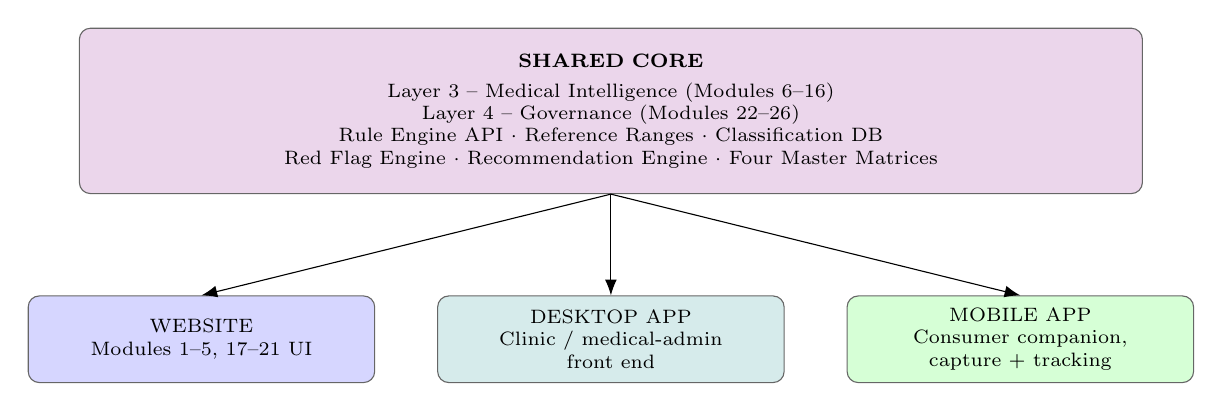
\begin{tikzpicture}[>=Latex]
\node[draw=black!60,rounded corners,fill=violet!16,minimum width=13.5cm,minimum height=2.1cm,align=center,font=\scriptsize,text width=13.25cm,inner sep=2pt] (core) at (0,0) {\textbf{SHARED CORE}\\[3pt]Layer 3 -- Medical Intelligence (Modules 6--16)\\Layer 4 -- Governance (Modules 22--26)\\Rule Engine API $\cdot$ Reference Ranges $\cdot$ Classification DB\\Red Flag Engine $\cdot$ Recommendation Engine $\cdot$ Four Master Matrices};
\node[draw=black!60,rounded corners,fill=blue!16,minimum width=4.4cm,minimum height=1.1cm,align=center,font=\scriptsize,text width=4.15cm,inner sep=2pt] (web) at (-5.2,-2.9) {WEBSITE\\Modules 1--5, 17--21 UI};
\node[draw=black!60,rounded corners,fill=teal!16,minimum width=4.4cm,minimum height=1.1cm,align=center,font=\scriptsize,text width=4.15cm,inner sep=2pt] (desk) at (0,-2.9) {DESKTOP APP\\Clinic / medical-admin\\front end};
\node[draw=black!60,rounded corners,fill=green!16,minimum width=4.4cm,minimum height=1.1cm,align=center,font=\scriptsize,text width=4.15cm,inner sep=2pt] (mob) at (5.2,-2.9) {MOBILE APP\\Consumer companion,\\capture + tracking};
\draw[-{Latex[length=2mm]}] (core.south)--(web.north);
\draw[-{Latex[length=2mm]}] (core.south)--(desk.north);
\draw[-{Latex[length=2mm]}] (core.south)--(mob.north);
\end{tikzpicture}
\end{adjustbox}
\end{center}
\end{frame}

\section{Website Version}

\begin{frame}[t]{Website Version -- Structure}
\textcolor{black!55}{\scriptsize Modules 1--5, 17--21 (UX) over the shared rule-engine backend}\\[2pt]
\begin{itemize}
\scriptsize
\item Primary Version 1 channel: fastest to iterate, no install, launches the full end-to-end patient flow
\item Registration $\to$ profile $\to$ blood report upload $\to$ rule engine $\to$ targeted questions $\to$ report $\to$ follow-up
\item Covers Phase 1 (Metabolic / Cardiovascular) first, per the framework's phased rollout
\end{itemize}
\vspace{4pt}
\begin{center}
\begin{adjustbox}{max width=0.96\linewidth,max height=0.62\textheight}
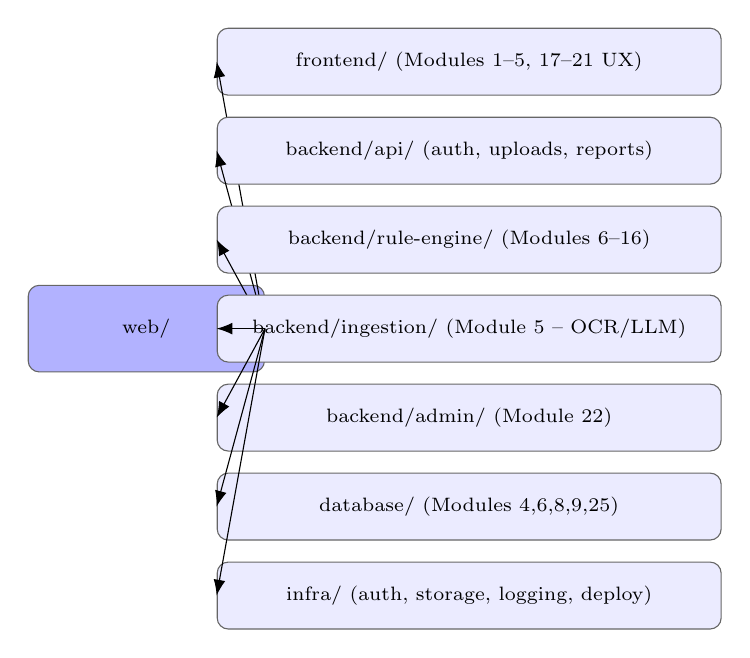
\begin{tikzpicture}[>=Latex]
\node[draw=black!60,rounded corners,fill=blue!30,minimum width=3.0cm,minimum height=1.1cm,align=center,font=\scriptsize,text width=2.75cm,inner sep=2pt] (wsc) at (0,-3.3900000000000006) {web/};
\node[draw=black!60,rounded corners,fill=blue!8,minimum width=6.4cm,minimum height=0.85cm,align=center,font=\scriptsize,text width=6.15cm,inner sep=2pt] (ws0) at (4.1,0) {frontend/  (Modules 1--5, 17--21 UX)};
\draw[-{Latex[length=2mm]}] (wsc.east)--(ws0.west);
\node[draw=black!60,rounded corners,fill=blue!8,minimum width=6.4cm,minimum height=0.85cm,align=center,font=\scriptsize,text width=6.15cm,inner sep=2pt] (ws1) at (4.1,-1.13) {backend/api/  (auth, uploads, reports)};
\draw[-{Latex[length=2mm]}] (wsc.east)--(ws1.west);
\node[draw=black!60,rounded corners,fill=blue!8,minimum width=6.4cm,minimum height=0.85cm,align=center,font=\scriptsize,text width=6.15cm,inner sep=2pt] (ws2) at (4.1,-2.26) {backend/rule-engine/  (Modules 6--16)};
\draw[-{Latex[length=2mm]}] (wsc.east)--(ws2.west);
\node[draw=black!60,rounded corners,fill=blue!8,minimum width=6.4cm,minimum height=0.85cm,align=center,font=\scriptsize,text width=6.15cm,inner sep=2pt] (ws3) at (4.1,-3.3899999999999997) {backend/ingestion/  (Module 5 -- OCR/LLM)};
\draw[-{Latex[length=2mm]}] (wsc.east)--(ws3.west);
\node[draw=black!60,rounded corners,fill=blue!8,minimum width=6.4cm,minimum height=0.85cm,align=center,font=\scriptsize,text width=6.15cm,inner sep=2pt] (ws4) at (4.1,-4.52) {backend/admin/  (Module 22)};
\draw[-{Latex[length=2mm]}] (wsc.east)--(ws4.west);
\node[draw=black!60,rounded corners,fill=blue!8,minimum width=6.4cm,minimum height=0.85cm,align=center,font=\scriptsize,text width=6.15cm,inner sep=2pt] (ws5) at (4.1,-5.6499999999999995) {database/  (Modules 4,6,8,9,25)};
\draw[-{Latex[length=2mm]}] (wsc.east)--(ws5.west);
\node[draw=black!60,rounded corners,fill=blue!8,minimum width=6.4cm,minimum height=0.85cm,align=center,font=\scriptsize,text width=6.15cm,inner sep=2pt] (ws6) at (4.1,-6.779999999999999) {infra/  (auth, storage, logging, deploy)};
\draw[-{Latex[length=2mm]}] (wsc.east)--(ws6.west);
\end{tikzpicture}
\end{adjustbox}
\end{center}
\end{frame}

\begin{frame}[t]{Website Version -- Technology Stack}
\textcolor{black!55}{\scriptsize One language family per side of the stack, minimal moving parts}\\[2pt]
\begin{center}\scriptsize
\begin{tabular}{p{3.6cm}p{9.5cm}}
\toprule
\textbf{Layer} & \textbf{Recommendation} \\
\midrule
Frontend & TypeScript + React (Next.js) -- server-rendered marketing pages, client-rendered assessment wizard \\
Backend / Rule Engine & Python (FastAPI) -- strong fit for the rule engine, clean path to ML/OCR, typed schemas via Pydantic \\
Database & PostgreSQL -- Module 25's structured objects map directly to relational tables \\
Async / background jobs & Python + task queue (e.g. Celery) -- OCR extraction and report generation off the request path \\
Admin console (Module 22) & Same React/TypeScript stack, gated behind medical-admin roles (Module 25) \\
\bottomrule
\end{tabular}
\end{center}
\end{frame}

\begin{frame}[t]{Website Version -- Key Features}
\textcolor{black!55}{\scriptsize Extraction intelligence, rule fidelity, and admin control}\\[2pt]
\begin{itemize}
\scriptsize
\item \textbf{LLM/OCR blood-report extraction} -- image/PDF upload $\to$ OCR $\to$ LLM-assisted mapping into structured \{test, result, unit, reference range\} records against the Lab Test Master Database (Module 6); AI assists extraction and wording only, never classification (framework Section 27)
\item Rule-engine API implementing Modules 6--16 exactly as documented, never duplicated client-side
\item Unit conversion service (Module 7) so results from different labs are comparable
\item Report generator with PDF/print export (Module 19)
\item Medical admin console (Module 22) -- edit reference ranges, classifications, triggers, recommendation wording without a redeploy
\item Auth, consent and role-based access (Modules 1, 25); audit/version logging (Modules 23--24) surfaced per report
\end{itemize}
\end{frame}

\section{Desktop App Version}

\begin{frame}[t]{Desktop App Version -- Structure}
\textcolor{black!55}{\scriptsize Shares the website's UI kit; adds offline intake and admin tooling}\\[2pt]
\begin{itemize}
\scriptsize
\item Positioned as the \textbf{clinic / medical-professional and administration channel}, not a second consumer app
\item Best fit for bulk/administrative rule management, and clinics where connectivity or IT policy favour a local-first tool
\end{itemize}
\vspace{4pt}
\begin{center}
\begin{adjustbox}{max width=0.96\linewidth,max height=0.62\textheight}
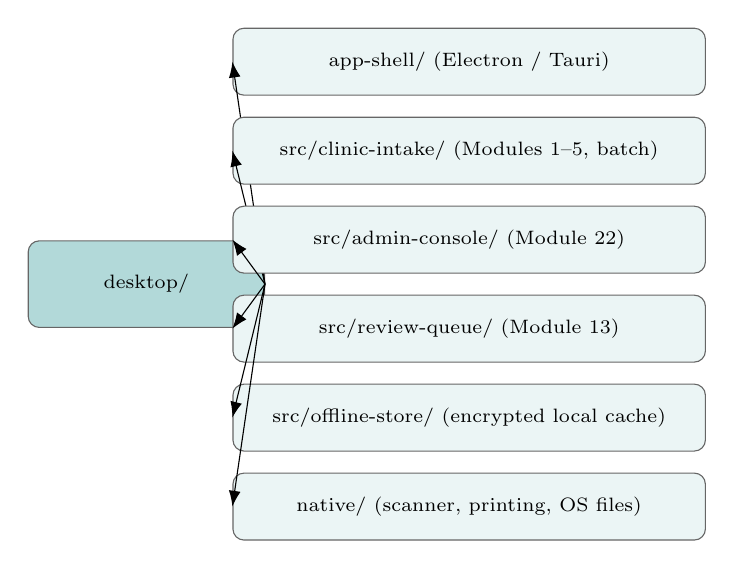
\begin{tikzpicture}[>=Latex]
\node[draw=black!60,rounded corners,fill=teal!30,minimum width=3.0cm,minimum height=1.1cm,align=center,font=\scriptsize,text width=2.75cm,inner sep=2pt] (dsc) at (0,-2.825) {desktop/};
\node[draw=black!60,rounded corners,fill=teal!8,minimum width=6.0cm,minimum height=0.85cm,align=center,font=\scriptsize,text width=5.75cm,inner sep=2pt] (ds0) at (4.1,0) {app-shell/  (Electron / Tauri)};
\draw[-{Latex[length=2mm]}] (dsc.east)--(ds0.west);
\node[draw=black!60,rounded corners,fill=teal!8,minimum width=6.0cm,minimum height=0.85cm,align=center,font=\scriptsize,text width=5.75cm,inner sep=2pt] (ds1) at (4.1,-1.13) {src/clinic-intake/  (Modules 1--5, batch)};
\draw[-{Latex[length=2mm]}] (dsc.east)--(ds1.west);
\node[draw=black!60,rounded corners,fill=teal!8,minimum width=6.0cm,minimum height=0.85cm,align=center,font=\scriptsize,text width=5.75cm,inner sep=2pt] (ds2) at (4.1,-2.26) {src/admin-console/  (Module 22)};
\draw[-{Latex[length=2mm]}] (dsc.east)--(ds2.west);
\node[draw=black!60,rounded corners,fill=teal!8,minimum width=6.0cm,minimum height=0.85cm,align=center,font=\scriptsize,text width=5.75cm,inner sep=2pt] (ds3) at (4.1,-3.3899999999999997) {src/review-queue/  (Module 13)};
\draw[-{Latex[length=2mm]}] (dsc.east)--(ds3.west);
\node[draw=black!60,rounded corners,fill=teal!8,minimum width=6.0cm,minimum height=0.85cm,align=center,font=\scriptsize,text width=5.75cm,inner sep=2pt] (ds4) at (4.1,-4.52) {src/offline-store/  (encrypted local cache)};
\draw[-{Latex[length=2mm]}] (dsc.east)--(ds4.west);
\node[draw=black!60,rounded corners,fill=teal!8,minimum width=6.0cm,minimum height=0.85cm,align=center,font=\scriptsize,text width=5.75cm,inner sep=2pt] (ds5) at (4.1,-5.6499999999999995) {native/  (scanner, printing, OS files)};
\draw[-{Latex[length=2mm]}] (dsc.east)--(ds5.west);
\end{tikzpicture}
\end{adjustbox}
\end{center}
\end{frame}

\begin{frame}[t]{Desktop App Version -- Technology Stack}
\textcolor{black!55}{\scriptsize Reuses the website's React code; adds a native shell and local store}\\[2pt]
\begin{center}\scriptsize
\begin{tabular}{p{3.6cm}p{9.5cm}}
\toprule
\textbf{Layer} & \textbf{Recommendation} \\
\midrule
Shell & Tauri (Rust shell + the same TypeScript/React UI) -- smaller install, lower memory; Electron (Node.js + TS) as fallback for faster native-module access \\
Shared UI & TypeScript + React -- same component library as the website, one design system for both \\
Local storage & SQLite, encrypted at rest -- offline queueing, syncs to PostgreSQL via the same Rule Engine API \\
Native integrations & Rust (Tauri commands) or Node native modules -- scanner / printer access \\
\bottomrule
\end{tabular}
\end{center}
\end{frame}

\begin{frame}[t]{Desktop App Version -- Key Features}
\textcolor{black!55}{\scriptsize The admin console is arguably desktop's biggest differentiator}\\[2pt]
\begin{itemize}
\scriptsize
\item \textbf{Offline-first intake} -- clinics with unreliable internet register patients and enter/scan reports locally; results sync and pass through the shared Rule Engine once online
\item Scanner / printer integration for physical blood reports and for printing the final report (Module 19)
\item Batch processing -- multiple patients' reports queued and processed together
\item Medical admin console (Module 22) as a first-class feature -- edit reference ranges, classifications, red flags, recommendation content; review/approve/publish versioning (Module 23) with an audit trail (Module 24)
\item Red-flag review queue (Module 13) -- dashboard for clinical staff to triage escalated cases
\item Role-based permissions distinguishing medical admin, clinic staff and read-only reviewer accounts (Module 25)
\end{itemize}
\end{frame}

\section{Mobile App Version}

\begin{frame}[t]{Mobile App Version -- Structure}
\textcolor{black!55}{\scriptsize Capture-and-track, on the same API contract as web and desktop}\\[2pt]
\begin{itemize}
\scriptsize
\item The \textbf{consumer companion}: makes the two most-repeated actions frictionless -- capturing a new blood report, checking progress
\item Carries the longitudinal-tracking and follow-up experience (Modules 17, 20, 21) that a one-time website visit does not serve well
\end{itemize}
\vspace{4pt}
\begin{center}
\begin{adjustbox}{max width=0.96\linewidth,max height=0.62\textheight}
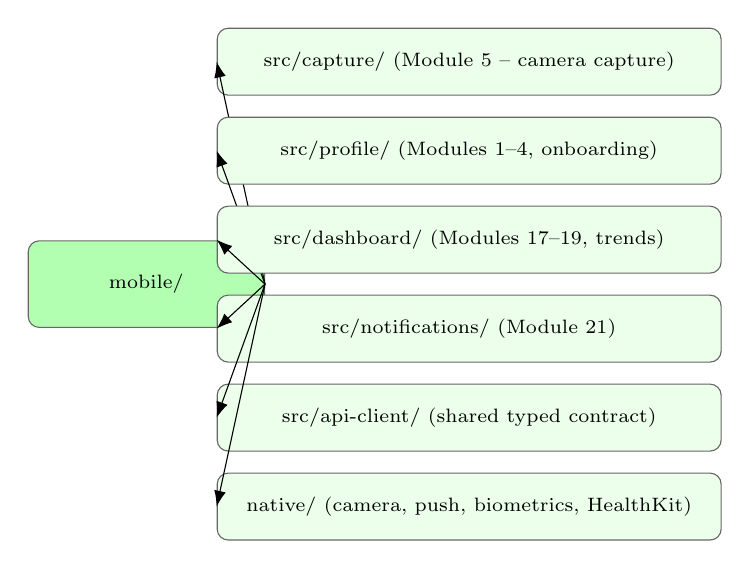
\begin{tikzpicture}[>=Latex]
\node[draw=black!60,rounded corners,fill=green!30,minimum width=3.0cm,minimum height=1.1cm,align=center,font=\scriptsize,text width=2.75cm,inner sep=2pt] (mbc) at (0,-2.825) {mobile/};
\node[draw=black!60,rounded corners,fill=green!8,minimum width=6.4cm,minimum height=0.85cm,align=center,font=\scriptsize,text width=6.15cm,inner sep=2pt] (mb0) at (4.1,0) {src/capture/  (Module 5 -- camera capture)};
\draw[-{Latex[length=2mm]}] (mbc.east)--(mb0.west);
\node[draw=black!60,rounded corners,fill=green!8,minimum width=6.4cm,minimum height=0.85cm,align=center,font=\scriptsize,text width=6.15cm,inner sep=2pt] (mb1) at (4.1,-1.13) {src/profile/  (Modules 1--4, onboarding)};
\draw[-{Latex[length=2mm]}] (mbc.east)--(mb1.west);
\node[draw=black!60,rounded corners,fill=green!8,minimum width=6.4cm,minimum height=0.85cm,align=center,font=\scriptsize,text width=6.15cm,inner sep=2pt] (mb2) at (4.1,-2.26) {src/dashboard/  (Modules 17--19, trends)};
\draw[-{Latex[length=2mm]}] (mbc.east)--(mb2.west);
\node[draw=black!60,rounded corners,fill=green!8,minimum width=6.4cm,minimum height=0.85cm,align=center,font=\scriptsize,text width=6.15cm,inner sep=2pt] (mb3) at (4.1,-3.3899999999999997) {src/notifications/  (Module 21)};
\draw[-{Latex[length=2mm]}] (mbc.east)--(mb3.west);
\node[draw=black!60,rounded corners,fill=green!8,minimum width=6.4cm,minimum height=0.85cm,align=center,font=\scriptsize,text width=6.15cm,inner sep=2pt] (mb4) at (4.1,-4.52) {src/api-client/  (shared typed contract)};
\draw[-{Latex[length=2mm]}] (mbc.east)--(mb4.west);
\node[draw=black!60,rounded corners,fill=green!8,minimum width=6.4cm,minimum height=0.85cm,align=center,font=\scriptsize,text width=6.15cm,inner sep=2pt] (mb5) at (4.1,-5.6499999999999995) {native/  (camera, push, biometrics, HealthKit)};
\draw[-{Latex[length=2mm]}] (mbc.east)--(mb5.west);
\end{tikzpicture}
\end{adjustbox}
\end{center}
\end{frame}

\begin{frame}[t]{Mobile App Version -- Technology Stack}
\textcolor{black!55}{\scriptsize Cross-platform by default, native where capture quality demands it}\\[2pt]
\begin{center}\scriptsize
\begin{tabular}{p{3.6cm}p{9.5cm}}
\toprule
\textbf{Layer} & \textbf{Recommendation} \\
\midrule
App framework & TypeScript + React Native -- maximises code/type-sharing with the website's React/TS codebase and API client; Flutter (Dart) is a reasonable alternative if native rendering performance is prioritised over code-sharing \\
Native modules & Camera / OCR pre-processing (crop, enhance) in Swift/Kotlin invoked from React Native, or a cross-platform camera library where sufficient \\
Local storage & Encrypted on-device store (e.g. SQLite/Realm) -- offline viewing of the last report and cached trends \\
Push notifications & APNs / FCM -- drives Module 21 follow-up and repeat-test reminders \\
\bottomrule
\end{tabular}
\end{center}
\end{frame}

\begin{frame}[t]{Mobile App Version -- Key Features}
\textcolor{black!55}{\scriptsize The capture channel that proves OCR/LLM quality daily}\\[2pt]
\begin{itemize}
\scriptsize
\item \textbf{Camera-based capture + LLM/OCR extraction} -- photograph a paper or PDF report, run the same extraction pipeline as the website, confirm low-confidence values (Module 3 validation) before entering the rule engine
\item Push notifications for follow-up (Module 21) -- ``repeat HbA1c in 3 months,'' ``update your weight,'' ``your next report is due''
\item Trend dashboard (Module 17) -- e.g. ``Your HbA1c has shown a progressive upward trend across three measurements,'' with simple charts
\item Biometric login for fast, secure repeat access to sensitive health data
\item Optional HealthKit / Health Connect integration -- weight, activity, blood pressure feed Modules 3--4 automatically where the user opts in
\item Offline report viewing -- last report and trend history available without connectivity
\end{itemize}
\end{frame}

\section{Suggested Build Sequence}

\begin{frame}[t]{Suggested Build Sequence}
\textcolor{black!55}{\scriptsize Web first, then admin tooling, then desktop, then mobile, then scope expansion}\\[2pt]
\begin{itemize}
\scriptsize
\item Follows the framework's own phasing guidance: build one clinical domain at a time, not all 26 modules simultaneously
\item Each later clinical-domain expansion only touches the shared rule engine and matrices -- not platform-specific work
\end{itemize}
\vspace{4pt}
\begin{center}
\begin{adjustbox}{max width=0.96\linewidth,max height=0.6\textheight}
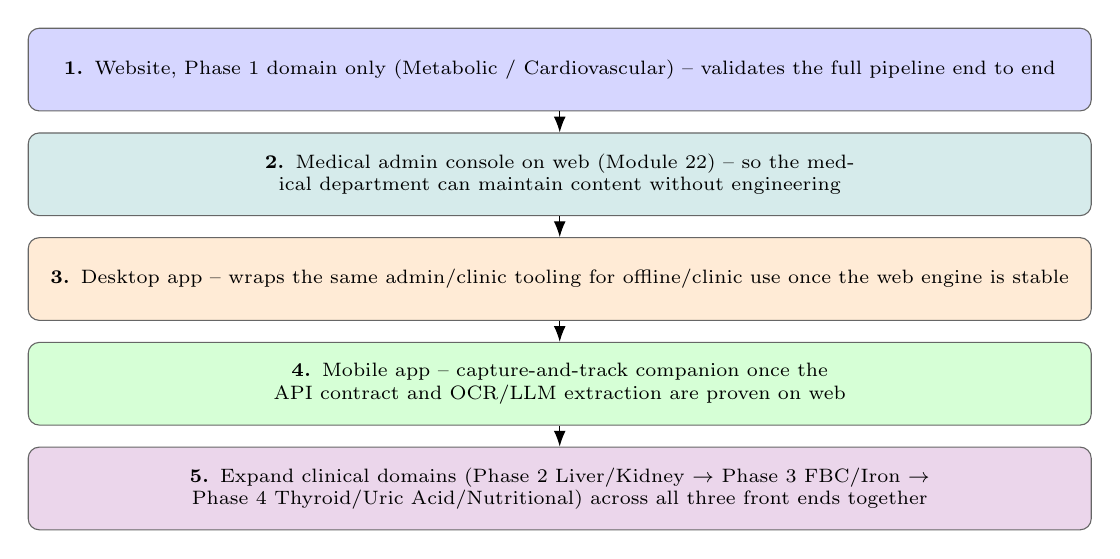
\begin{tikzpicture}[>=Latex]
\node[draw=black!60,rounded corners,fill=blue!16,minimum width=13.5cm,minimum height=1.05cm,align=center,font=\scriptsize,text width=13.25cm,inner sep=2pt] (lv0) at (0,0) {\textbf{1.} Website, Phase 1 domain only (Metabolic / Cardiovascular) -- validates the full pipeline end to end};
\node[draw=black!60,rounded corners,fill=teal!16,minimum width=13.5cm,minimum height=1.05cm,align=center,font=\scriptsize,text width=13.25cm,inner sep=2pt] (lv1) at (0,-1.33) {\textbf{2.} Medical admin console on web (Module 22) -- so the medical department can maintain content without engineering};
\node[draw=black!60,rounded corners,fill=orange!16,minimum width=13.5cm,minimum height=1.05cm,align=center,font=\scriptsize,text width=13.25cm,inner sep=2pt] (lv2) at (0,-2.66) {\textbf{3.} Desktop app -- wraps the same admin/clinic tooling for offline/clinic use once the web engine is stable};
\node[draw=black!60,rounded corners,fill=green!16,minimum width=13.5cm,minimum height=1.05cm,align=center,font=\scriptsize,text width=13.25cm,inner sep=2pt] (lv3) at (0,-3.99) {\textbf{4.} Mobile app -- capture-and-track companion once the API contract and OCR/LLM extraction are proven on web};
\node[draw=black!60,rounded corners,fill=violet!16,minimum width=13.5cm,minimum height=1.05cm,align=center,font=\scriptsize,text width=13.25cm,inner sep=2pt] (lv4) at (0,-5.32) {\textbf{5.} Expand clinical domains (Phase 2 Liver/Kidney $\to$ Phase 3 FBC/Iron $\to$ Phase 4 Thyroid/Uric Acid/Nutritional) across all three front ends together};
\draw[-{Latex[length=2mm]}] (lv0.south)--(lv1.north);
\draw[-{Latex[length=2mm]}] (lv1.south)--(lv2.north);
\draw[-{Latex[length=2mm]}] (lv2.south)--(lv3.north);
\draw[-{Latex[length=2mm]}] (lv3.south)--(lv4.north);
\end{tikzpicture}
\end{adjustbox}
\end{center}
\end{frame}

\section{Medical Department Execution Plan}

\begin{frame}[t]{Medical Department Execution Plan -- Eight Steps}
\textcolor{black!55}{\scriptsize Scope $\to$ draft $\to$ review $\to$ hand-off $\to$ test $\to$ publish $\to$ monitor $\to$ repeat}\\[2pt]
\begin{itemize}
\scriptsize
\item The medical logic person owns Modules 6--16 plus the medical content of Modules 22--24 -- in practice, the Four Master Matrices
\item Sequenced so engineering is never blocked on undefined medical content, and nothing ships without clinical sign-off
\item The medical department stays one phase ahead of engineering rather than becoming a bottleneck
\end{itemize}
\vspace{4pt}
\begin{center}
\begin{adjustbox}{max width=0.96\linewidth,max height=0.58\textheight}
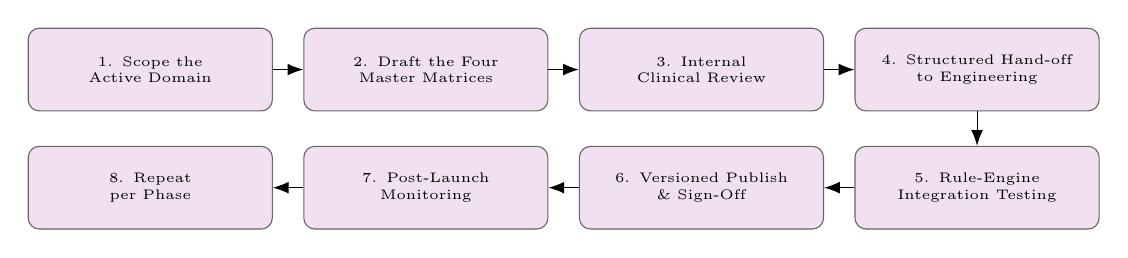
\begin{tikzpicture}[>=Latex]
\node[draw=black!60,rounded corners,fill=violet!12,minimum width=3.1cm,minimum height=1.05cm,align=center,font=\tiny,text width=2.85cm,inner sep=2pt] (s0) at (0.0,0.0) {1. Scope the\\Active Domain};
\node[draw=black!60,rounded corners,fill=violet!12,minimum width=3.1cm,minimum height=1.05cm,align=center,font=\tiny,text width=2.85cm,inner sep=2pt] (s1) at (3.5,0.0) {2. Draft the Four\\Master Matrices};
\node[draw=black!60,rounded corners,fill=violet!12,minimum width=3.1cm,minimum height=1.05cm,align=center,font=\tiny,text width=2.85cm,inner sep=2pt] (s2) at (7.0,0.0) {3. Internal\\Clinical Review};
\node[draw=black!60,rounded corners,fill=violet!12,minimum width=3.1cm,minimum height=1.05cm,align=center,font=\tiny,text width=2.85cm,inner sep=2pt] (s3) at (10.5,0.0) {4. Structured Hand-off\\to Engineering};
\node[draw=black!60,rounded corners,fill=violet!12,minimum width=3.1cm,minimum height=1.05cm,align=center,font=\tiny,text width=2.85cm,inner sep=2pt] (s4) at (10.5,-1.5) {5. Rule-Engine\\Integration Testing};
\node[draw=black!60,rounded corners,fill=violet!12,minimum width=3.1cm,minimum height=1.05cm,align=center,font=\tiny,text width=2.85cm,inner sep=2pt] (s5) at (7.0,-1.5) {6. Versioned Publish\\\& Sign-Off};
\node[draw=black!60,rounded corners,fill=violet!12,minimum width=3.1cm,minimum height=1.05cm,align=center,font=\tiny,text width=2.85cm,inner sep=2pt] (s6) at (3.5,-1.5) {7. Post-Launch\\Monitoring};
\node[draw=black!60,rounded corners,fill=violet!12,minimum width=3.1cm,minimum height=1.05cm,align=center,font=\tiny,text width=2.85cm,inner sep=2pt] (s7) at (0.0,-1.5) {8. Repeat\\per Phase};
\draw[-{Latex[length=2mm]}] (s0.east)--(s1.west);
\draw[-{Latex[length=2mm]}] (s1.east)--(s2.west);
\draw[-{Latex[length=2mm]}] (s2.east)--(s3.west);
\draw[-{Latex[length=2mm]}] (s3.south)--(s4.north);
\draw[-{Latex[length=2mm]}] (s4.west)--(s5.east);
\draw[-{Latex[length=2mm]}] (s5.west)--(s6.east);
\draw[-{Latex[length=2mm]}] (s6.west)--(s7.east);
\end{tikzpicture}
\end{adjustbox}
\end{center}
\end{frame}

\begin{frame}[t]{The Four Master Matrices}
\textcolor{black!55}{\scriptsize The brain of MyHealthReport -- Step 2 of the execution plan}\\[2pt]
\begin{itemize}
\scriptsize
\item Every matrix entry carries a \texttt{RULE\_ID}, guideline/source citation and version tag from the outset -- this becomes the audit trail in Module 24
\item Delivered as structured data (spreadsheet or admin console), never prose -- the practical enforcement of ``never hard-code medical knowledge into the front end''
\item Safety Matrix (C) entries are specifically checked against \textbf{Safety Override $>$ Wellness Recommendation}
\end{itemize}
\vspace{4pt}
\begin{center}
\begin{adjustbox}{max width=0.96\linewidth,max height=0.58\textheight}
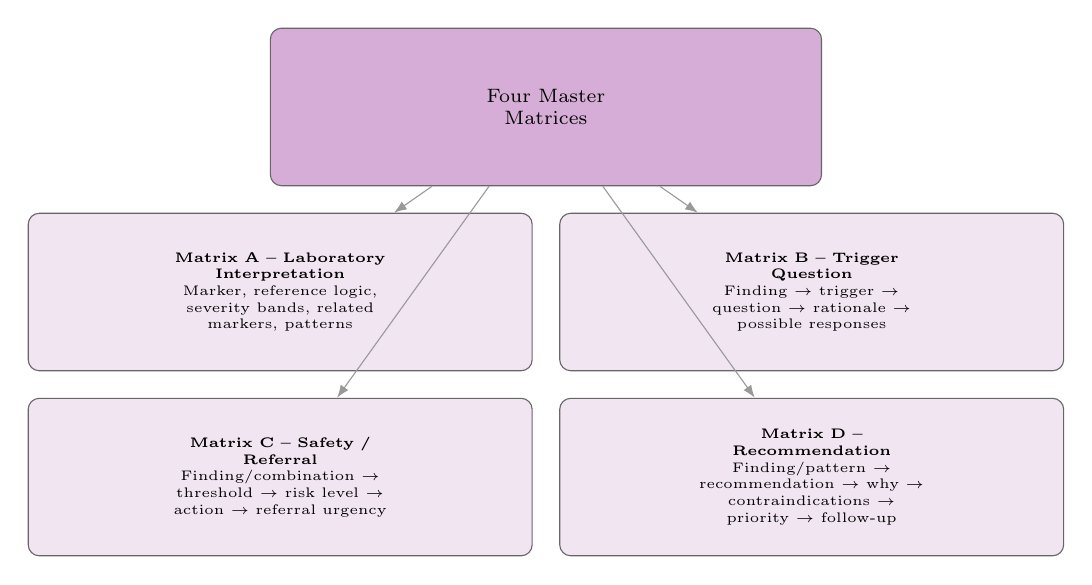
\begin{tikzpicture}[>=Latex]
\node[draw=black!60,rounded corners,fill=violet!10,minimum width=6.4cm,minimum height=2.0cm,align=center,font=\tiny,text width=6.15cm,inner sep=2pt] (g0) at (0.0,0.0) {\textbf{Matrix A -- Laboratory}\\\textbf{Interpretation}\\Marker, reference logic,\\severity bands, related\\markers, patterns};
\node[draw=black!60,rounded corners,fill=violet!10,minimum width=6.4cm,minimum height=2.0cm,align=center,font=\tiny,text width=6.15cm,inner sep=2pt] (g1) at (6.75,0.0) {\textbf{Matrix B -- Trigger}\\\textbf{Question}\\Finding $\to$ trigger $\to$\\question $\to$ rationale $\to$\\possible responses};
\node[draw=black!60,rounded corners,fill=violet!10,minimum width=6.4cm,minimum height=2.0cm,align=center,font=\tiny,text width=6.15cm,inner sep=2pt] (g2) at (0.0,-2.35) {\textbf{Matrix C -- Safety /}\\\textbf{Referral}\\Finding/combination $\to$\\threshold $\to$ risk level $\to$\\action $\to$ referral urgency};
\node[draw=black!60,rounded corners,fill=violet!10,minimum width=6.4cm,minimum height=2.0cm,align=center,font=\tiny,text width=6.15cm,inner sep=2pt] (g3) at (6.75,-2.35) {\textbf{Matrix D --}\\\textbf{Recommendation}\\Finding/pattern $\to$\\recommendation $\to$ why $\to$\\contraindications $\to$\\priority $\to$ follow-up};
\node[draw=black!60,rounded corners,fill=violet!32,minimum width=7.0cm,minimum height=2.0cm,align=center,font=\scriptsize,text width=6.75cm,inner sep=2pt] (gc) at (3.375,2.35) {Four Master\\Matrices};
\draw[-{Latex[length=1.6mm]},black!40] (gc)--(g0);
\draw[-{Latex[length=1.6mm]},black!40] (gc)--(g1);
\draw[-{Latex[length=1.6mm]},black!40] (gc)--(g2);
\draw[-{Latex[length=1.6mm]},black!40] (gc)--(g3);
\end{tikzpicture}
\end{adjustbox}
\end{center}
\end{frame}


\begin{frame}
\centering
\Huge Thank You
\vspace{10pt}

\normalsize \textit{MyHealthReport --- Platform Structure \& Execution Plan}
\end{frame}

\end{document}
